\graphicspath{{./images/}}

\chapter{Ausgangslage}

\section{Ist-Zustand}

Die Applikation MEON ist seit x.x.x in Betrieb und wird aktuell gewartet und weiterentwickelt. Die Applikation wurde unter speziellen Bedienungen im Zuge von der beiden DevOps Initiativen HAKA6 und SuperSonic \footnote{Firmeninterne Programme bei denen es um die Einführung von DevOps Praktiken geht} umgesetzt, so dass gewisse Technologien mit Unterstützung dieser Initiativen benutzt werden durften, die zu diesem Zeitpunkt noch nicht produktiv betrieben wurden. Der Marktdruck und die Initiativen ermöglichten eine enge Zusammenarbeit zwischen Business und Entwicklung, bei welcher die Anforderungen zusammen erarbeitet wurden und ohne formalen Dokumente direkt vom Product Owner ins Team gegeben wurden, weshalb keine entsprechenden Requirements Dokumente vorliegen.

\subsection{Technisch}

Die Applikation wurde mit aktuellen Frameworks entwickelt. In der folgenden Tabelle sind die wichtigsten Komponenten und ihre Funktionen kurz aufgelistet.

\begin{table}[H]
	\centering
	\caption{Technische Rahmenbedienungen}
	\begin{tabular}{ | p{4cm} | p{12cm} | }
		\toprule
		{\textbf{Technologie / Tool}} & {\textbf{Einsatzzweck}} \\
		\midrule
		Java 8 & Die Serverapplikation ist damit implementiert und wird deshalb wieder verwendet. \\ \hline
		Java Script & Der Webapplikation ist damit implementiert und wird deshalb wieder verwendet. \\ \hline
		Spring Framework & Dient als Basisframework für den Serverteil der Applikation.  \\ \hline
		AngularJS & Webframework für die Webapplikation. \\ \hline
		Docker & Deployment der einzelnen Teile der Applikation als Container. \\ \hline
		JBoss 10 & Applikations Server welcher die Laufzeitumgebung für die Applikation bereitstellt. \\ \hline
		Apache Webserver & HTTP Server für den statischen Inhalt. \\ \hline
		Camunda BPM & Workflow-Management-System welches die Prozesse für die Anmeldung eines neuen Händlers steuert. \\ \hline
		RDBMS: Oracle, MySQL / NoSQL: MongoDB & Speichern der Daten. \\
		\bottomrule
	\end{tabular}
\end{table}

Die Anwendung ist technologisch auf einem sehr modernen Stand. Der Einsatz der Containertechnologie Docker hat sich bewährt und wird auch in anderen Projekten eingesetzt. Ob der weitere Einsatz von JBoss respektive Applikationserver weiterhin notwending ist, kann zur Disposition gestellt werden. Dies vor allem durch die teilweise Unklarheit der Stossrichtung der Java Enterprise Edition. Obschon Oracle mitterweile Pläne vorgelegt hat, sind nicht alle Zweifel über die Zukunft ausgeräumt. Da die Applikation bereits auf Spring basiert könnte hier der Schritt Richtung Spring Boot mit verhältnismässig geringem Aufwand durchgeführt werden.

Im folgenden Bild ist die Architektur von MEON abgebildet.

\begin{center}
	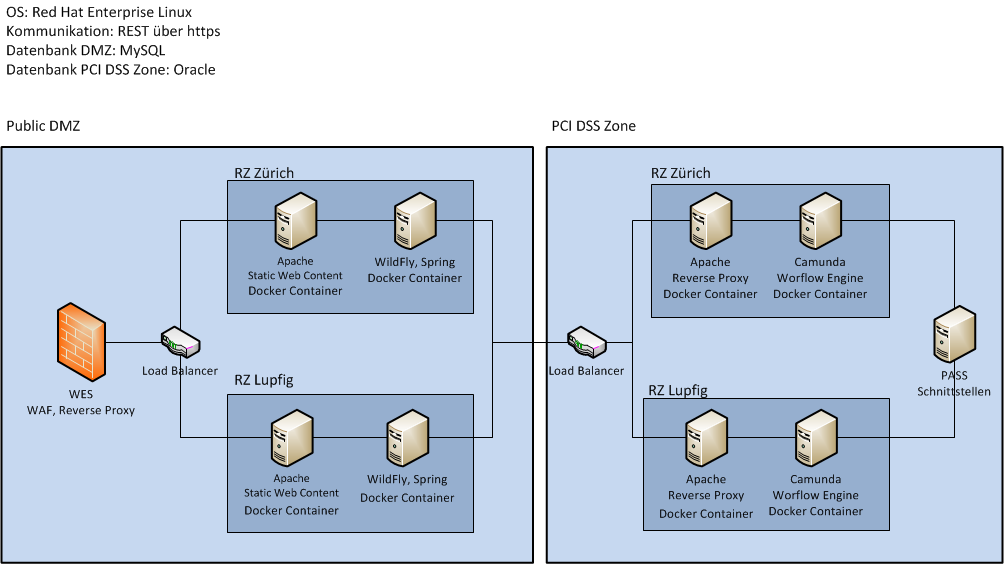
\includegraphics[scale=0.55]{meon_arch.png}
\end{center}
\textcolor {red}{Verstehe den folgenden Paragraphen nicht, da fehlt meiner Meinung nach was}
Die Applikation ist in einer entspricht eher einer klassischen Schichtenarchitektur wobei diese nicht auf dem gleichen System laufen sondern in separaten Containern ausgeliefert werden. Die Architektur hat sich aktuell bewährt. 

\subsection{Organisatorisch}

Da \textcolor{red} {SIX wird ohne Artikel verwendet, irgendwo im Intranet gibt es ein entsprechendes Dokument fürs Wording} SIX im Finanzbereich tätig ist, gibt es entsprechende Richtlinien und Prozesse wann, wie und ob Änderungen überhaupt in Produktion gehen dürfen. Aktuell werden die Changes im Issue Trackingsystem Jira erfasst und mit einer Release Version versehen. Durch die Anbindung an Fisheye und SVN ist jederzeit ersichtlich mit welchem Ticket welche Codeteile betroffen waren. Da das Projekt unter lockeren Bedienungen umgesetzt wurde ist ein Eintrag im ITSM \footnote{Change Management Applikation welche für das Erfassen von Änderungen an Systemem verwendet wird.} System aktuell nicht Pflicht obschon das gemäss normalen Richtlinien der Fall wäre. \textcolor {red} {}Ein entsprechender Prozess aus dem Jira ins ITSM ist bereits umgesetzt und kann angesteuert werden, so dass alles in einem Tool ersichtlich ist. }
Gemäss den Richtlinien müsste eine Änderung fünf Personentage vor Going live eingetragen und freigegeben sein. Die Praxis ist wie erwähnt auf die Branche der SIX zurück zu führen und hat unter genauerer Betrachtung auch eher formellen Nutzen. Die Freigabe im System wir meistens von Personen gemacht welche gar nicht an der Entwicklung und Betrieb der Applikation beteiligt sind. Daher ist auch eine Beurteilung der Änderungen gar nicht möglich. Hier wäre wohl eine Kategorisierung der Applikation, welche einen solchen Prozess benötigen, sinnvoll um nicht unnötige Prozesse für kleine nicht zwingen kritische Applikation zu forcieren.

\section{Situationsanalyse}

SIX befindet sich aktuell im Bezug auf Betrieb und Entwicklung von Applikationen im Wandel. Bereits erwähnte DevOps Initiativen laufen und werden von immer mehr Projekten angewendet, ja sogar gelebt. In diesem Zug ist aktuell auch eine OpenShift 3 \footnote{Software welche eine Cloud Umgebung für Container bereitstellt. Als Container Technologie wird Docker verwendent. Für die Orchestration der Container, wird Kubernetes von Google verwendet.} Installation im Gange, welche die Bereitstellung neuer Applikationen mit einem Cloud Ansatz noch weiter vereinfachen soll.
Durch die Initiativen ändert sich auch der organisatorische Aspekt. So sollen Value Streams erschaffen werden, in welchen eine End-To-End Verantwortung für Applikation wahrgenommen wird und entscheide dezentral gefällt werden können. Insbesondere das Change Management muss sich zur Zeit an die neuen Methoden gewöhnen und damit umgehen lernen.

\section{Methoden}

\subsection{Scrum}

Für das Projekt Management der Masterthesis wird Scrum\footnote{Iteratives Entwicklungsverfahren welches sich auf das Agile Manifesto stützt und diesem diverse Rollen hinzufügt. } verwendet. Im Rahmen der Masterthesis wird jedoch nicht der ganze Werkzeugkasten der Methode verwendet da dies zuviel Aufwand bedeuten würde. Wichtige Teile wie das Planning werden entsprechen kurz gehalten.
Scrum eignet sich gut für die Umsetztung der Arbeit da es impliziet einen kurzen Feedbackzyklus vorschreibt. Da es sich beim Thema für SIX um Neuland handelt und daher keine Erfahrungen vorliegen, sind kleine iterative Schritte gut um Risiken früh zu erkennen und Anpassungen schnell umzusetzen.

\subsection{Prototyping}
Die neu entstehende Architektur soll auf ihre Tauglichkeit verifiziert werden. Da die Applikation bereits in Betrieb ist und aktuell stark erweitert wird, soll die Umsetzung mittels Prototyping geprüft werden. Hierbei werden die, aus Architektursicht kritischen Bestandteile und deren Technologien und Prinzipien getestet. Für das automatische Testing stehen bereits Mockimplemetationen zu Verfügung, welche ebenfalls in den Prototypen verwendet werden kann. Dadurch kann schnell eine Aussage über die Verwendbarkeit getroffen werden. 
